\section{Implementation} \label{sec:implementation}
In this section, we dive deep into our label flipping algorithms using a methodical approach that starts with a study of the base code dissected in Section \ref{sec:base_code}. In order to lay the foundation for our hypotheses, this first step involves disassembling the existing components and exploring the rationale behind their design decisions.

On the basis of this fundamental knowledge, we present a number of novel concepts aimed towards improving and extending label flipping techniques. To push the limits of effectiveness and applicability, each modification is motivated by a strategic vision that combines theoretical insights with practical considerations.

These improvements, which range from new ideas to small modifications, collectively aim to refine and enhance the overall performance of the label flipping attacks. Through careful implementation and rigorous testing, we seek to demonstrate the efficacy of our approach and highlight the evolution of label flipping algorithms into more sophisticated and effective tools for adversarial scenarios. The implemented code can be accessed on the project's GitHub repository \cite{MastersThesisCode}.

For the upcoming results, which will be detailed in Section \ref{sec:results}, our focus revolves around devising attacks that optimize four parameters:
\begin{itemize}
        \item Test error (TE). Error resulting from the loss function used in training. The lower TE, the better.
        \item Overall accuracy (All-Acc). Number of correct predictions divided by the total number of predictions for all the examples. The greater All-Acc, the better.
        \item Source class accuracy (Src-Acc). Number of the source class examples correctly predicted divided by the total number of the source class examples. The greater Src-Acc, the better.
        \item Attack success rate (ASR). Proportion of the source class examples incorrectly classified as the target class. Since we aim to attack the system, the higher ASR, the better.
\end{itemize}

\subsection{Chosen parameters and modifications}\label{sec:chosen_parameters}
The first step after dissecting the base code \cite{LFighter_code} is to choose the parameters that we use for our experiments:
\begin{itemize}
        \item Independent and Identically Distributed (IID) data: In an IID case, all the peers have a uniform sample of the data, meaning each peer possesses a similar proportion of each class. Thus, each of them represents a proportion of the global data. As a result, every update they compute serves as an unbiased estimate of the global model. In the non-IID scenario, this is not the case. Each user could have different percentages of classes or contain many outliers or various other scenarios. In the most extreme case, each user might only have data corresponding to a single class. In such instances, the updates computed by peers can be significantly dissimilar from one another. 
        
        IID is the simpler case for defences, and therefore more challenging for attackers. If an attack performs moderately well in the IID case, it should perform better in the non-IID case. Or, at the very least, it should be harder to detect. That is why it makes sense to start here. The non-IID case would be the most favourable scenario, as many defences will likely fail directly. The reality is that peers typically fall somewhere in between: neither fully IID nor completely non-IID. The IID case serves as a good starting point for research into these topics.
        \item Global rounds: This variable is set to 100. This means that the global model is updated 100 times.
        \item Local epochs\footnote{Epochs refer to the quantity of iterations a ML algorithm performs on the entire training dataset. Each epoch involves the algorithm making incremental adjustments to its model parameters based on the training data, aiming to improve its performance over time.}: This variable is set to 3. This means that each peer trains its model for 3 epochs before sending the update to the server.
        \item Number of peers: There are 20 peers in the system. 
\end{itemize}
We first began using the MNIST dataset for our experiments because it is the most common dataset used in the literature. However, we quickly realized that the results were not very interesting. The reason for this is that the MNIST dataset is too simple. The model is able to achieve a very high accuracy, and the label flipping attacks are not able to reduce it significantly. Therefore, we decided to use the CIFAR-10 dataset instead. This dataset is more complex, and the model is not able to achieve such a high accuracy. This means that the label flipping attacks are able to reduce the accuracy significantly. In the following sections, we present the results obtained with the MNIST dataset along with the ones obtained with the CIFAR-10 dataset. The reason behind this is to show the difference between both datasets. However, we focus on the results obtained with the CIFAR-10 dataset because they are more interesting. Our aim will be to flip the labels of the source class (dog) to the target class label (cat). 

Another minimal change made to the base code is adding a condition checking if the device being used for the experiments is a Graphics Processing Unit (GPU) or the device's Central Processing Unit (CPU). This change is made because the GPU is much faster than the CPU when employing tensors\footnote{Tensors are multi-dimensional arrays commonly used in mathematics and machine learning to represent data. In machine learning, tensors are used to store and manipulate data, such as images, sequences, and more complex structures. Tensors are particularly well-suited for ML tasks due to their ability to efficiently handle large volumes of data and perform operations in parallel. GPUs are highly effective for tensor operations, as they are optimized for parallel computing.}. The code used to perform this check is shown in \autoref{listing:gpu_check}.

Finally, we also added a section after the FL system has finished the global rounds to print the results obtained in a confusion matrix format. This matrix is a table that is often used to describe the performance of a classification model on a set of test data for which the true values are known. The code used to print this matrix is shown in \autoref{listing:confusion_matrix_code}.

\begin{listing}[h]
        \begin{minted}
        [
            autogobble,
            breaklines,
            breakautoindent,
            % highlightlines={1, 3-4},
            linenos
        ]
        {python}
        import torch
        ...
        if torch.cuda.is_available():
                DEVICE = "cuda"
                print('GPU is available:', torch.cuda.get_device_name(0))
        else:
                DEVICE = "cpu"
                print('GPU is not available, CPU will be used')
        DEVICE = torch.device(DEVICE)
        ...
        \end{minted}
    
        \caption{Computing device selection and information}
        \label{listing:gpu_check}
    \end{listing}

\begin{listing}[h]
        \begin{minted}
        [
            autogobble,
            breaklines,
            breakautoindent,
            % highlightlines={1, 3-4},
            linenos
        ]
        {python}
        from matplotlib import pyplot as plt
        ...
        actuals, predictions = self.test_label_predictions(simulation_model, self.device, self.test_loader, dataset_name=self.dataset_name)
        plt.matshow(confusion_matrix(actuals, predictions))
        plt.colorbar()
        plt.show()
        ...
        \end{minted}

        \caption{Printing the confusion matrix}
        \label{listing:confusion_matrix_code}
\end{listing}

%%%%%%%%%%%%%%%%%%%%%%%%%%%%%%%%%%%%%%%%%%%%%%%%%%%%%%%%%%%%%%%
\subsection{Main structure of the hypotheses code}
In order to test our hypotheses, we first have to design how the code will be structured. The main idea is to have an if-statement for each hypothesis inside the \textit{participant\_update()} function, as commented in Section \ref{sec:base_code}. This condition will contain all the code needed to perform the label flipping attack. The code will be structured as follows:
\begin{enumerate}
        \item The first step is to iterate through the local model's samples.
                \begin{enumerate}
                        \item For each sample, we have to check if the sample's label is the source class's label. If it is, we must keep its index in a list.
                        \item After that, we have to make any calculation needed in order to obtain some kind of punctuation to give to each sample. This punctuation will be used to determine which samples will be flipped.
                \end{enumerate}
        \item Joining the index list with the punctuation list. This is helpful because we can sort the list by the punctuation and then flip the labels of the samples with the highest punctuation.
        \item Determining which samples to flip based on the punctuation obtained in the previous step.
        \item Flipping the labels of the samples selected in the previous step, given their indices.
        \item Loading the new dataset with the flipped labels into the dataset used to train the local model.
\end{enumerate}

%%%%%%%%%%%%%%%%%%%%%%%%%%%%%%%%%%%%%%%%%%%%%%%%%%%%%%%%%%%%%%%
\subsection{Standard label flipping}\label{sec:standard_label_flipping}
This is the label flipping algorithm that is used in the base code \cite{LFighter_code}. It is a very simple algorithm that flips the labels of all the samples of the source class to the target class's label.

When analysing how this algorithm works, we realize that it cannot be included in our solution as is. This is because, in a very intelligent way, it flips all the source class's labels by looping through the indices of all the samples, checking if they belong to the source class and then, flips them. As it has been stated before, our purpose is to flip a subset of these labels. Therefore, we have to devise a new algorithm that allows us to flip only the selected samples' labels. This presents us with an opportunity to craft a more targeted and sophisticated approach that aligns precisely with our objectives.

%%%%%%%%%%%%%%%%%%%%%%%%%%%%%%%%%%%%%%%%%%%%%%%%%%%%%%%%%%%%%%%
\subsection{Entropy-based label flipping}\label{sec:entropy_label_flipping}
The first algorithm we propose is based on the entropy of the samples. The entropy is a measure of the uncertainty of a random variable. In this case, the random variable is the label of the sample. \autoref{fig:high_vs_low_entropy} shows the clear difference between a high and low entropy. The samples with a high entropy are the ones that are more difficult to classify, while the samples with a low entropy are the ones that are easier to classify.

\begin{figure}[h]
        \centering
        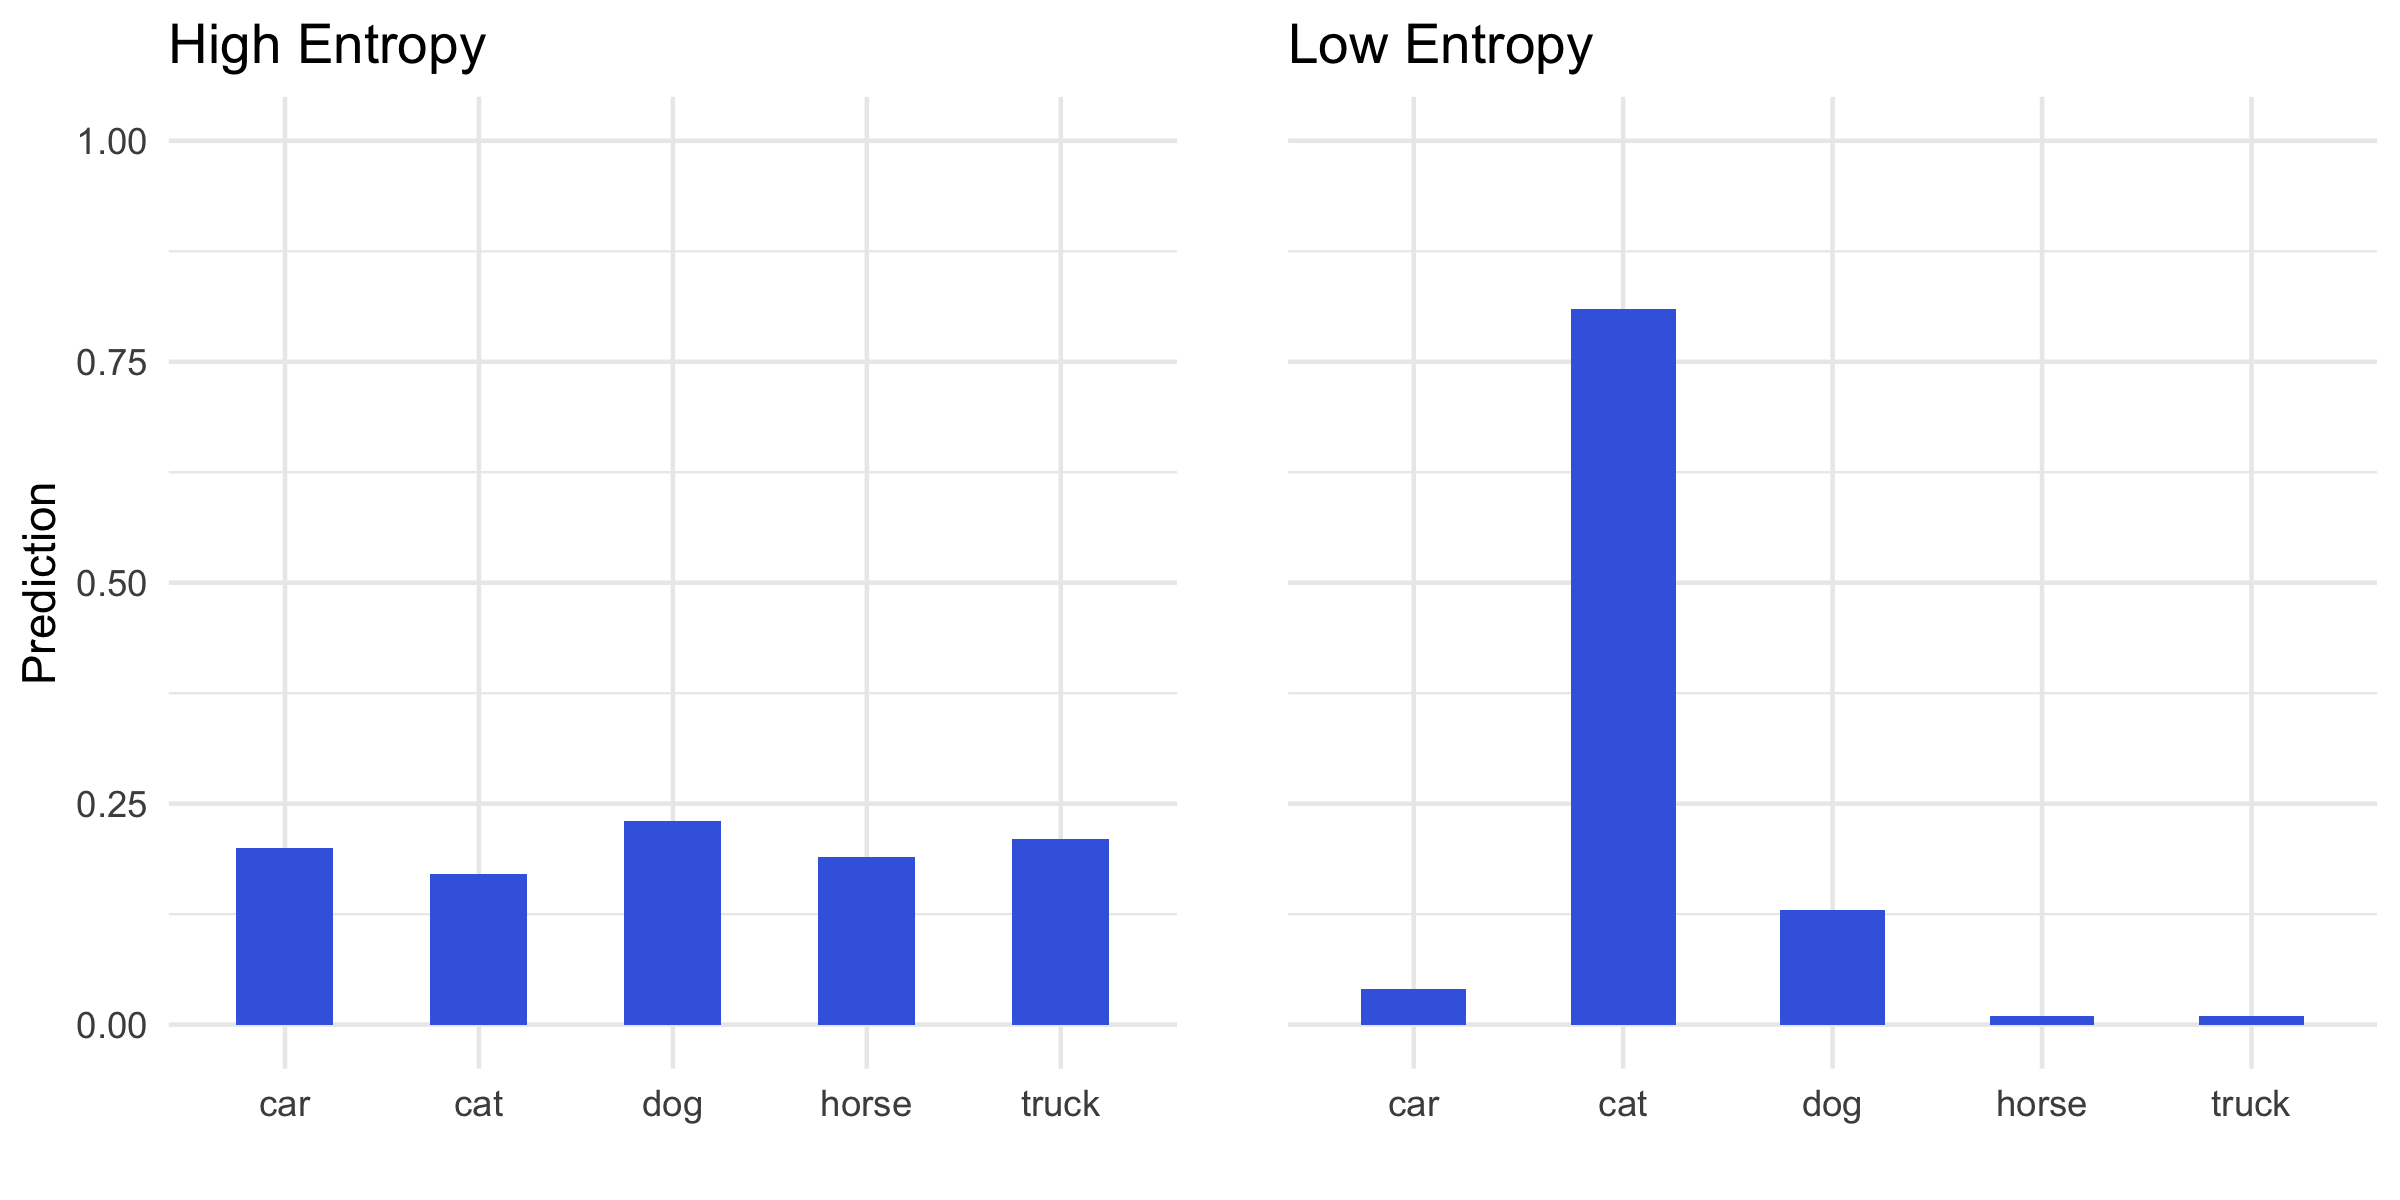
\includegraphics[scale=0.18]{high_vs_low_entropy.png}
        \caption{High vs. low entropy}
        \label{fig:high_vs_low_entropy}
\end{figure}

Therefore, our first approach is to flip the labels of the samples with a high entropy because they are the ones that are more likely to be misclassified. The structure that this algorithm follows is the next one and the code is shown in \autoref{listing:entropy_label_flipping_code}:
\begin{enumerate}
        \item Initialize empty lists to store the indices of the samples of the source class and the entropy associated with each sample.
        \item Iterate through the local model's samples using the DataLoader\footnote{A "DataLoader" in PyTorch refers to a utility class that simplifies the process of loading and managing data for training and testing machine learning models.}.
                \begin{enumerate}
                        \item For each sample, we have to check if the sample's label is the source class's label. If it is, we append its index in the list. Since we iterate through batches of samples, it is important to keep the absolute index and not the relative one.
                        \item Then, we introduce the samples into a tensor so we can predict the output the model would return.
                        \item To obtain this output, we call the \textit{model(data\_source\_batch)} function.
                        \item After that, we must transform the output to NumPy\footnote{NumPy is a fundamental package in the Python programming language used for numerical computations and data manipulation. It provides support for working with large, multi-dimensional arrays and matrices, along with an extensive collection of mathematical functions to operate on these arrays efficiently.} format so we can calculate the entropy.
                        \item Finally, we to compute the entropy of the sample and store it in a list.
                \end{enumerate}
        \item We merge the indices and entropies lists into a single list.
        \item The next step is sorting the list by \textbf{highest entropy}.
        \item We select the top 50\% of the list.
        \item We sort it again by index, so we can flip the labels of the samples in the correct order as we iterate in the following step.
        \item To iterate through the samples in the local dataset, we create a \textit{index\_label\_flip()} function, shown in \autoref{listing:index_label_flip_code} in order to overcome the problem with the main flipping function mentioned in Section \ref{sec:standard_label_flipping}. This function works as follows:
                \begin{enumerate}
                        \item The function receives the dataset, the sorted indices and entropies list, and the target class (its ID).
                        \item It begins by the creation of an empty list to store the poisoned data.
                        \item Then, it iterates through the dataset.
                        \item For each sample, it checks if the sample's index is in the sorted indices list.
                        \item If it is, it appends a structure with the data of the sample and the target class's label to the poisoned data list.
                        \item If it is not, it appends a structure with the data of the sample and the original label to the poisoned data list.
                        \item Finally, it returns the poisoned data list.
                \end{enumerate}
        \item Next, we create a new DataLoader object with the poisoned dataset, ready to be used to train the local model.
        \item Finally, we increment a counter that keeps track of the number of attacks performed and print the information about the attack.
\end{enumerate}

\begin{listing}[H]
        \begin{minted}
        [
            autogobble,
            breaklines,
            breakautoindent,
            % highlightlines={1, 3-4},
            linenos
        ]
        {python}
        if (attack_type == 'entropy_label_flipping') and (self.peer_type == 'attacker'):
            train_loader = DataLoader(self.local_data, self.local_bs, shuffle = False, drop_last=True)
            model.eval()  # Set the model to evaluation mode
            entropies = []  # To store entropies for each data sample
            kept_indices=[] #to store the indices of the data samples with label==target_class
            with torch.no_grad():
                for batch_idx, (data, labels) in enumerate(train_loader):
                    # Find the indices of data samples with label of the source class
                    source_mask = labels == source_class
                    # Keep the positions of the data samples with label==source_class
                    kept_indices_batch = (batch_idx * train_loader.batch_size + i for i in range(len(source_mask)) if source_mask[i])
                    kept_indices.extend(kept_indices_batch)
                    # Get the data samples with label target
                    data_source_batch = data[source_mask]
                    # Send the data samples with label=source_class to the device
                    data_source_batch = data_source_batch.to(self.device)
                    # Obtain the predicted outputs for data samples with label source_class
                    output = model(data_source_batch)  # Get the model's output for the source class data samples
                    predictions_np=(output.cpu().numpy())   # Convert the output to numpy
                    entropies.extend(stats.entropy(predictions_np, axis=1)) # Entropy is calculated by row
            entropy_list = list(zip(kept_indices, entropies))
            sorted_entropy_list = sorted(entropy_list, key=lambda x: x[1], reverse=True)    # Sort it by entropy value
            num_elements_to_keep = len(sorted_entropy_list) // 2   # Number of elements that represents the 50% of the data that we can attack
            top_50_percent = sorted_entropy_list[:num_elements_to_keep] # Extract the top 50% of the data
            sorted_entropy_list = sorted(top_50_percent, key=lambda x: x[0])  # Sort by index to keep the order of the data
            
            poisoned_data = index_label_flip(train_loader.dataset, sorted_entropy_list, target_class)
            # Create a new DataLoader with the updated dataset and with a shuffle
            train_loader = DataLoader(poisoned_data, self.local_bs, shuffle = True, drop_last=True)
            self.performed_attacks+=1
            print('Entropy-based Label flipping attack launched')
        \end{minted}

        \caption{Entropy-based label flipping algorithm}
        \label{listing:entropy_label_flipping_code}
\end{listing}

It is important to note that the iterations through the DataLoader are not deterministic if the \textit{shuffle} parameter is set to true because each time we iterate through the DataLoader, the samples are shuffled. Our solution is to set the parameter to false before the first access so we can keep the indices of the samples in the same order to flip them. Then, after the dataset poisoning is completed, as we create the new DataLoader, we set the parameter to true again so the model does not learn the order of the samples.

\begin{listing}[H]
        \begin{minted}
        [
            autogobble,
            breaklines,
            breakautoindent,
            % highlightlines={1, 3-4},
            linenos
        ]
        {python}
        def index_label_flip(dataset, sorted_list, target_class):
                poisoned_data = []
                for i, (data, label) in enumerate(dataset):
                if i in [index for index, _ in sorted_list]:
                        poisoned_data.append((data, target_class))  # Change the label to target_class
                else:
                        poisoned_data.append((data, label))  # Keep the original label
                return poisoned_data
        \end{minted}

        \caption{\textit{index\_label\_flip()} function}
        \label{listing:index_label_flip_code}
\end{listing}

Given that the execution time for an attack with the parameters mentioned in Section \ref{sec:chosen_parameters} is approximately 4 hours for an Nvidia RTX2060 graphics card, and that we are executing eight attacks per poisoning method, as seen in Section \ref{sec:defenses}, we are not able to try all the possible modifications of the entropy-based label flipping attack. Therefore, we have to choose the ones that we think are the most promising. The modifications that we have chosen to implement and test are the following:
\begin{itemize}
        \item Keeping the highest 25\% entropies. This modification is based on the idea that the samples with the highest entropy are the ones that are more likely to be misclassified. Therefore, if we are more specific and only flip the labels of the samples with the highest entropy, we should be able to increase the attack success rate by avoiding detection from the server. To modify the code, we only have to change line 23 of \autoref{listing:entropy_label_flipping_code} to \textit{num\_elements\_to\_keep = len(sorted\_entropy\_list) // \textbf{4}}.
        \item Keeping the highest 75\% entropies. This modification is based on the opposite idea, that is, if the attack is avoiding detection when poisoning 50\% of the samples, we can try to increase the attack success rate by poisoning more samples.
        \item Keeping the lowest 50\% entropies. The thought for this idea is that the samples with the lowest entropy are the ones that are easier to classify. Therefore, if we flip these labels, we may be able to confuse the server in the first training rounds, and indirectly lean benevolent peers to misclassify the samples according to our will. To modify the code, we only have to change line 22 of \autoref{listing:entropy_label_flipping_code} to \textit{sorted\_entropy\_list = sorted(entropy\_list, key=lambda x: x[1], reverse=\textbf{False})} so the list is ordered by ascending entropy.
        \item Keeping the lowest 25\% entropies. The reason for this modification is the same as the previous one, but being more specific and only flipping the labels from the samples that better represent the source class.
        \item Applying a scaling factor to the weights before the update. This modification is based on literature proposals to ensure a successful attack, commented in Section \ref{sec:defenses}. The code used to implement this modification is shown in \autoref{listing:scaling_factor_code}. The code is located at the end of the \textit{participant\_update()} function to receive the trained local model.
\end{itemize}

\begin{listing}[H]
        \begin{minted}
        [
            autogobble,
            breaklines,
            breakautoindent,
            % highlightlines={1, 3-4},
            linenos
        ]
        {python}
        def scale_model(update, scale_factor):
                for key in update.keys():
                update[key] = (update[key].float() * scale_factor).long()
                return update
        ...
        if self.peer_type == 'attacker' and (attack_type == 'entropy_label_flipping' or attack_type == 'closeness_label_flipping'):
                update = scale_model(model.state_dict(), scale_factor = 1.1)
                model.load_state_dict(update)
        \end{minted}

        \caption{Scaling factor implementation}
        \label{listing:scaling_factor_code}
\end{listing}

The verification process to ensure the correct functionality of the entropy-based label flipping algorithm has been carried out with meticulous attention to detail. Extensive testing and validation procedures have been executed to ensure that the algorithm operates as intended. The different evaluations that have been used to evaluate the algorithm's behaviour and performance are listed below:
\begin{itemize}
        \item Printing the entropies list to ensure that the range of values is correct. Then, printing the length of the entropies list and the indices list to ensure that they have the same length.
        \item Printing the sorted entropy list to ensure that the list is sorted by descending entropy. Then, when the list is trimmed, printing it again to make sure it is ordered by index.
        \item Counting and printing the amount of source class labels before and after the poisoning to ensure that the number of samples with the source class label has been reduced by the number of elements in the sorted entropy list. Then, performing the same operation with the target class label to ensure that the number of samples with the target class label has been increased by the number of elements in the sorted entropy list.
\end{itemize}

This attack's code sets the base that is used for the rest of the attacks. Therefore, the testing process is the same and the code is mildly modified to adapt it to the new attack.

%%%%%%%%%%%%%%%%%%%%%%%%%%%%%%%%%%%%%%%%%%%%%%%%%%%%%%%%%%%%%%%
\subsection{Closeness-based label flipping}\label{sec:closeness_label_flipping}
The second proposed algorithm uses the concept of sample closeness, which serves as a metric to determine how closely a given sample aligns with classification as either the source class or the target class. \autoref{fig:high_vs_low_closeness} shows the clear difference between a high and low closeness. The samples with a high closeness are the ones that are likely to be classified as either the source or the target class, while the samples with a low closeness are the ones that are more likely to be classified as one of them.

\begin{figure}[h!]
        \centering
        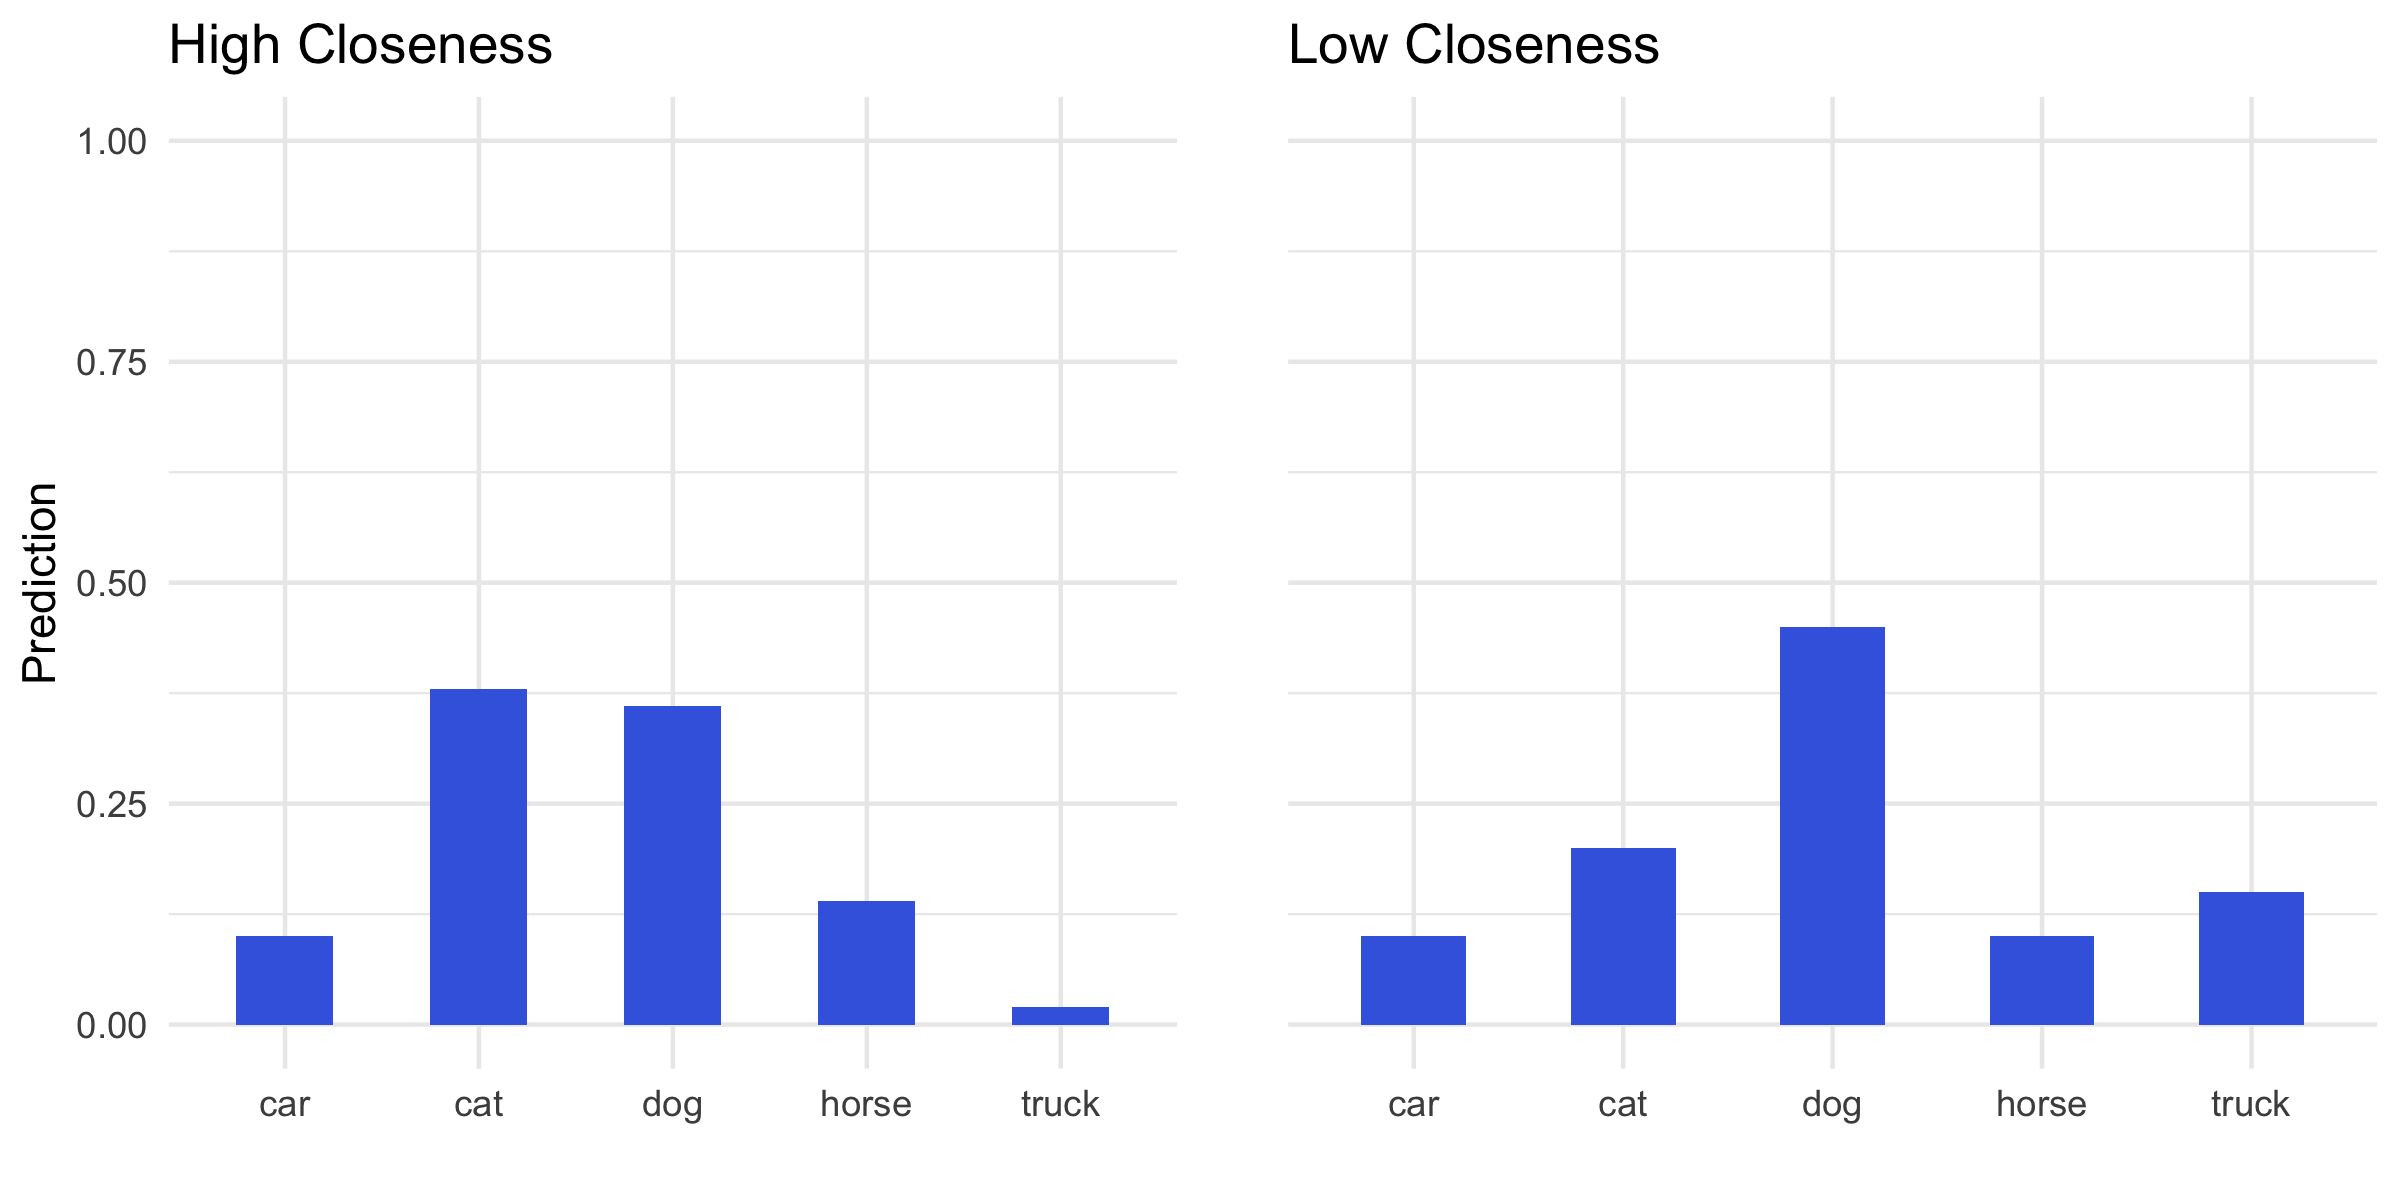
\includegraphics[scale=0.18]{high_vs_low_closeness.png}
        \caption{High vs. low closeness between classes \textit{dog} and \textit{cat}}
        \label{fig:high_vs_low_closeness}
\end{figure}

Hence, our strategy involves flipping the labels of samples exhibiting high closeness, as they are more likely to suffer potential misclassification. Another reason to choose high closeness is that the samples that have the higher closeness between the source and the target classes, may be also the ones more difficult to classify for the other peers. That could be, a dog with a short snout and hairy limbs that at first sight could be thought of as a cat.
The algorithm follows the subsequent structure, summarized since the logic is highly similar to the one explained in Section \ref{sec:entropy_label_flipping} and the corresponding code is provided in \autoref{listing:closeness_label_flipping_code}:
\begin{enumerate}
        \item Inside the main loop, iterating through the DataLoader, instead of calculating the entropy, we calculate the closeness between the source and the target class of the sample. This is done by calculating the absolute difference between the output of the model for the source class and the target class. The output is obtained by calling the \textit{model(data\_source\_batch)} function, as it was for the entropy solution.
        \item The following steps remain unchanged.
\end{enumerate}

\begin{listing}[h]
        \begin{minted}
        [
            autogobble,
            breaklines,
            breakautoindent,
            % highlightlines={1, 3-4},
            linenos
        ]
        {python}
        if (attack_type == 'closeness_label_flipping') and (self.peer_type == 'attacker'):
        ...
        closeness = []  # To store entropies for each data sample
        kept_indices=[] #to store the indices of the data samples with label==target_class
        with torch.no_grad():
        ...
                predictions_np=(output.cpu().numpy())   # Convert the output to numpy
                temp = []
                for i in range(len(predictions_np)):
                        temp.append(abs(predictions_np[i][source_class] - predictions_np[i][target_class]))
                closeness.extend(temp)
        ...
        \end{minted}

        \caption{Closeness-based label flipping algorithm}
        \label{listing:closeness_label_flipping_code}
\end{listing}
The set of different modifications that we have chosen to implement and test for the closeness-based label flipping attack are the following:
\begin{itemize}
        \item Keeping the highest 25\% closeness. This modification is based on the idea that the samples with the highest closeness are the ones that are more likely to be misclassified as the target class.
        \item Applying a threshold instead of keeping a percentage. The rationale behind this modification is that, as the global rounds progress, the global model is more refined. Therefore, the top percentage may include samples that are not as close to the target class as they were in the first global rounds. In order to mitigate this, we can try to keep the samples with a closeness difference, lower than a threshold. The code used to implement this modification is shown in \autoref{listing:threshold_code}. The code is located before the call to the \textit{index\_label\_flip()} function.
\end{itemize}

\begin{listing}[h]
        \begin{minted}
        [
            autogobble,
            breaklines,
            breakautoindent,
            % highlightlines={1, 3-4},
            linenos
        ]
        {python}
        ...
        sorted_closeness_list = sorted(closeness_list, key=lambda x: x[1])    # Sort it by entropy value
        threshold=0.02
        count=1
        actual=sorted_closeness_list[0][1]
        while actual <= threshold and count < len(sorted_closeness_list):
                count += 1
        num_elements_to_keep = count   # Number of elements that to keep
        top_closeness = sorted_closeness_list[:num_elements_to_keep]
        ...
        \end{minted}

        \caption{Threshold implementation}
        \label{listing:threshold_code}
\end{listing}
The verifications to test the correct functionality of the closeness-based label flipping algorithm are the same as the ones used for the entropy-based label flipping algorithm.

%%%%%%%%%%%%%%%%%%%%%%%%%%%%%%%%%%%%%%%%%%%%%%%%%%%%%%%%%%%%%%%
\subsection{Adaptive label flipping}\label{sec:adaptive_label_flipping}
The idea behind this approach is to use the previous two algorithms to create a more sophisticated and effective attack. The difference resides in the fact that, instead of using a fixed number of samples to flip, we use a percentage of the samples depending on how far the global model has been refined, taking into account the global rounds. The algorithm follows the subsequent structure, summarized since the logic is highly similar to the one explained in Section \ref{sec:entropy_label_flipping} and the corresponding code is provided in \autoref{listing:adaptive_label_flipping_code}:
\begin{enumerate}
        \item Before the main loop, we set an if statement to check if the global rounds are greater than the first defined segment. If they are, the loop will be the same as for either the closeness-based or the entropy-based label flipping algorithm. 
        \item Outside the loop, we will select the number of labels to flip depending on the global rounds. The idea is to flip a percentage of the samples that is inversely proportional to the global rounds. This means that, as the global rounds increase, the percentage of samples to flip decreases.
        \item If the current global round resides on the first segment, the code will be the same as for the standard label flipping algorithm. This means that all the source class labels will be flipped to the target class label.
\end{enumerate}



\begin{listing}[H]
        \begin{minted}
        [
            autogobble,
            breaklines,
            breakautoindent,
            % highlightlines={1, 3-4},
            linenos
        ]
        {python}
        if (attack_type == 'stealthy_closeness_label_flipping') and (self.peer_type == 'attacker'):
                ...
                if global_epoch > 25:
                        with torch.no_grad():
                                ...
                        sorted_entropy_list = sorted(entropy_list, key=lambda x: x[1], reverse=True)
                        num_elements_to_keep=0
                        if global_epoch <= 50:  # round 25 to 50, flip 75% of the data
                                num_elements_to_keep = len(sorted_entropy_list) // 2 + len(sorted_entropy_list) // 4
                        if global_epoch <= 75:  # round 50 to 75, flip 50% of the data
                                num_elements_to_keep = len(sorted_entropy_list) // 2
                        if global_epoch <= 100: # round 75 to 100, flip 25% of the data
                                num_elements_to_keep = len(sorted_entropy_list) //4
                        ...
                else:   # round 0 to 25, flip all the data
                        poisoned_data = label_filp(self.local_data, source_class, target_class)
                        train_loader = DataLoader(poisoned_data, self.local_bs, shuffle = True, drop_last=True)
                ...
        \end{minted}
        \caption{Adaptive label flipping algorithm}
        \label{listing:adaptive_label_flipping_code}
\end{listing}
The first segment does not follow the usual code because, since all the labels are flipped there is no point in computing the entropy or the closeness of the samples.

The set of different modifications that we have chosen to implement and test for the adaptive label flipping attack are the following:
\begin{itemize}
        \item Testing with entropy and closeness-based label flipping to  flip all the labels during the first half of the global rounds. During the second half, flip 50\% of the samples.
        \item Testing with either entropy or closeness-based label flipping to flip all the labels during the first half of the global rounds. During the second half, flip 25\% of the samples.
\end{itemize}

The verifications to test the correct functionality of the adaptive label flipping algorithm are the same as the ones used for the previous label flipping algorithms.

\pagebreak
